
\documentclass[aspectratio=169,10pt]{beamer}
\setbeamertemplate{navigation symbols}{\insertbackfindforwardnavigationsymbol}

\usetheme{Madrid}
\usecolortheme{default}

\makeatletter
\setbeamertemplate{footline}{%
  \leavevmode%
  \hbox{%
  \begin{beamercolorbox}[wd=.75\paperwidth,ht=2.25ex,dp=1ex,left,leftskip=0.3cm]{author in head/foot}%
    \fontsize{5}{6}\selectfont\insertshorttitle
  \end{beamercolorbox}%
  \begin{beamercolorbox}[wd=.25\paperwidth,ht=2.25ex,dp=1ex,right,rightskip=0.3cm]{date in head/foot}%
    \usebeamerfont{date in head/foot}\insertshortdate{}\hspace*{2em}
    \insertframenumber{}\,/\,\inserttotalframenumber\hspace*{2ex}
  \end{beamercolorbox}}%
  \vskip0pt%
}
\makeatother

% Core packages
\usepackage{amsmath,amssymb}
\usepackage{tikz-cd}
\usepackage{multicol}
\usepackage{algpseudocode}
\usepackage{booktabs}
\usepackage{graphicx}

\title{Discriminative Prompt Rerouting and Query Prototype Refinement on
Calibrated Prototype in Frozen Few Shot Class Incremental Learning}

\begin{document}

\begin{frame}
\begin{center}
    
\includegraphics[width=0.08\linewidth]{IUT.png}

    \vspace{0.8em}
    {\large \textbf{Discriminative Prompt Rerouting and Query Prototype Refinement on
Calibrated Prototype in Frozen Few Shot Class Incremental Learning}}

    \vspace{1.2em}
    {Md Akib Haider --- \textbf{210041222}}

    \vspace{0.3em}
    {Fateen Noor Rafee --- \textbf{210041120}}

    \vspace{0.3em}
    {Hasib Altaf --- \textbf{210041102}}

    \vspace{1.5em}
    \textbf{Supervised by}\\
    Reaz Hassan Joarder\\
    Junior Lecturer, Computer Vision Lab\\
    Department of Computer Science \& Engineering\\
    Islamic University of Technology
\end{center}
\end{frame}


\begin{frame}{Introduction: FSCIL Problem Formulation}



    \begin{columns}[c]
        \column{0.52\textwidth}
            \begin{block}{}
        N class of abundant images, K shots of new class images. Classification Problem
    \end{block}
        \vspace{0.4em}
        \begin{itemize}
            \item Base session have many classes ($>=$100), many sample images per class
            \item Incremental session introduces new (novel) classes each having K(=5) labeled images 
            \item Class sets across incremental sessions are mutually exclusive (called support sets)
            \item Old session data is inaccessible once training moves on
            \item Tested on unseen unlabeled query batch images
        \end{itemize}

        \column{0.45\textwidth}
        \centering
        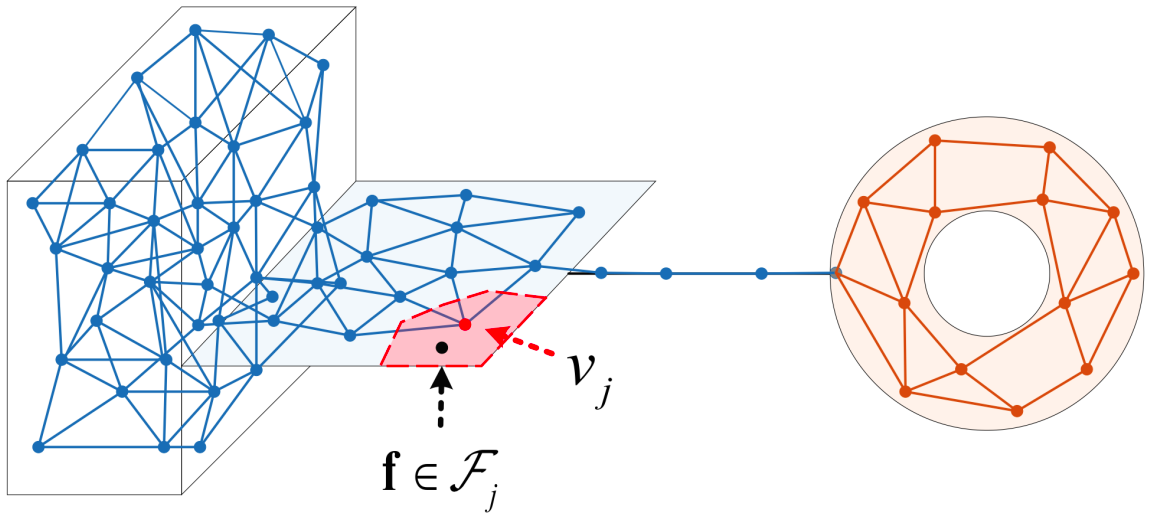
\includegraphics[width=\linewidth]{1 lit rev1 fscil.png}

        {\tiny Figure-1: Base and Novel Class Prototypes in Feature Space visualization}
    \end{columns}
\end{frame}


\begin{frame}{Motivation: FSCIL Challenges}
    \vfill
    \begin{itemize}
        \setlength{\itemsep}{1em}
        \item \textbf{Catastrophic forgetting}: adapting to new classes overwrites representations learned for earlier classes, whereas focusing on possibly noisy support set forgets base prototypes.
        \item \textbf{Overfitting}: only 5 samples/class makes novel-class estimates unstable (Chen et al., CVPR'25).
        \item \textbf{Intransigence}:  preserving knowledge from abundant existing classes from a highly limited
dataset.
        \item \textbf{Stability-plasticity tradeoff}: continual fine-tuning chases plasticity (ability to learn new things) but forgets; incremental-session freezing buys stability (ability to preserve what already learnt) but sacrifices plasticity.
        \item \textbf{Risk of noisy prototypes}: No guard mechanism of noisy support set images.
    \end{itemize}
    \vfill
\end{frame}

% \begin{frame}{Literature Review: OrCo (Orthogonality and Contrasive Loss)}


%     \begin{columns}[c]
%         \column{0.52\textwidth}
%         \vspace{0.4em}
%         \begin{itemize}
%             \item Pretraining with supervised and self-supervised contrasive learning enabling the model to capture various types of semantic information that is particularly beneficial for the novel classes
%             \item After pretraining, generate and fix mutually orthogonal random vectors (pseudotargets) and align the fixed pretrained backbone to the pseudo-targets using abundant base data
%             \item Learning objective: OrCo loss (PSCL + Feature orthogonality enforcer + standard CEL) to align the model with the pseudo-targets, using only few-shot from incremental sessions
%         \end{itemize}

%         \column{0.45\textwidth}
%         \centering
%         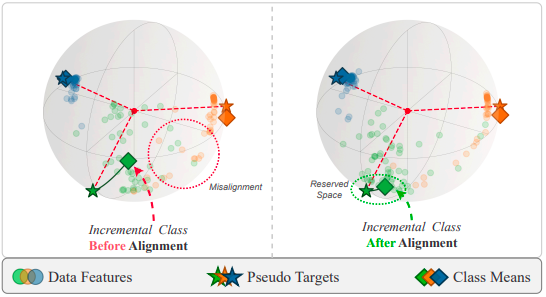
\includegraphics[width=\linewidth]{2 litrev2 orco.png}
%     \end{columns}

% \end{frame}

% \begin{frame}{Literature Review: OrCo (Orthogonality and Contrasive Loss)}

%         \begin{block}{}
%             \begin{itemize}
%                 \item Pretraining both backbone and projection head with SCL and SSCL in first phase 
%                 \item Projection head learnable parameters in both base and incremental sessions on next two phases 
%             \end{itemize}
%         \end{block}

%         \vspace{0.4em}


%         \centering
%         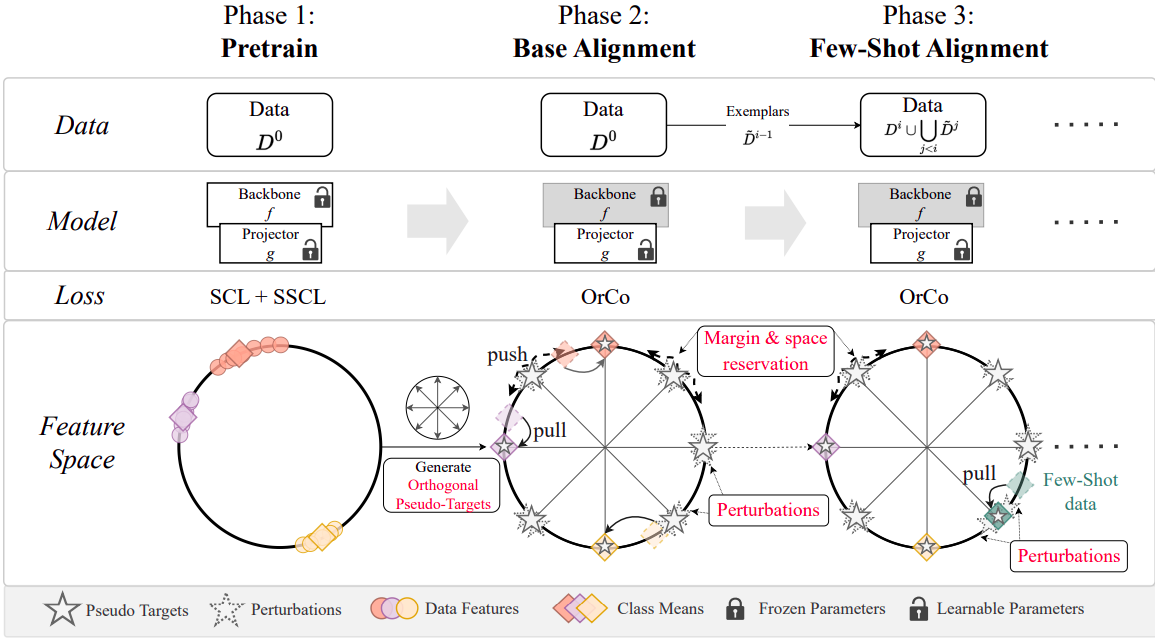
\includegraphics[width=0.7\linewidth]{3lit_rev_orco.png}

% \end{frame}


\begin{frame}{Literature Review: CEC (Continually Evolved Classifiers)   [2](CVPR, 2021)}


    \begin{columns}[c]
        \column{0.45\textwidth}
        \vspace{0.4em}
        {\footnotesize
        \begin{itemize}
            \item First, CEC trains a CNN backbone using the large base-class images and freeze the backbone 
            \item Problem? - Classifiers from different sessions don't know about each other (Session 0 learns Cat, Dog forgets Tiger, Lion from session 1)
            \item Treat each class classifier weight as nodes in graph; learn relationship between all class nodes (Graph Attention network)
            \item Create preudo new classes (augmentation) from base classes to train the GAT; better generalization, better classification on novel class (Continual Pseudo Incremental Learning)
        \end{itemize}
        }

        \column{0.54\textwidth}
        \centering
        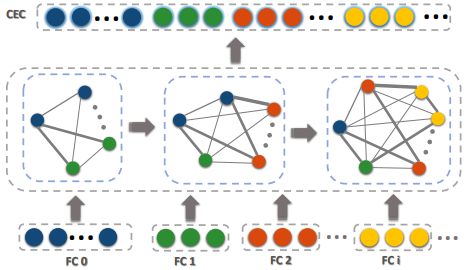
\includegraphics[width=\linewidth]{4_litrev_cec.png}

        {\tiny Figure-2: CEC graph model to adapt the classifier weights learned on individual sessions for the prediction over all classes}
    \end{columns}

\end{frame}


\begin{frame}{Literature Review: CEC (contd)   [2](CVPR, 2021)}

        \begin{block}{}
            \begin{itemize}
                \item Pretraining to learn the backbone model using training data in base session
                \item Pseudo incremental learning stage trains the graph model, require learnable parameters
                \item Classifier learning and adaptation stage uses support set (projection head weight update)
            \end{itemize}
        \end{block}

        \vspace{0.4em}


        \centering
        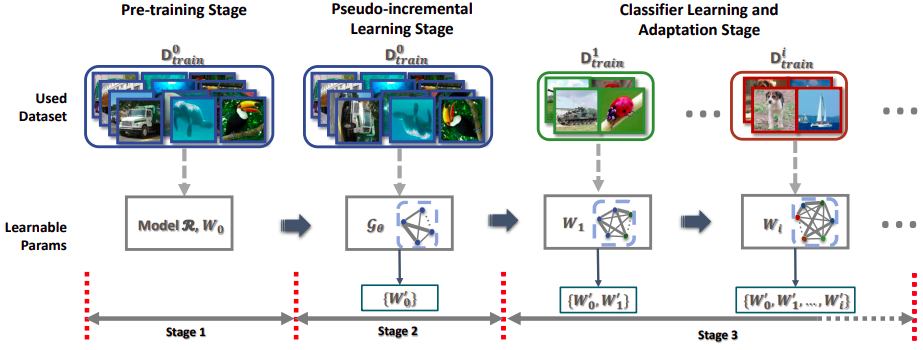
\includegraphics[width=0.8\linewidth]{5_lrcec.png}

        {\tiny Figure-3: Pretraining the backbone for continual learning stages in CEC architecture}

\end{frame}

\begin{frame}{Literature Review: RKD (Relation Knowledge Distillation) [3](AAAI, 2021)}

    \begin{columns}[c]
        \column{0.48\textwidth}
        {\footnotesize
        \begin{itemize}
            \item Individual knowledge distillation (IKD) forces each old sample near its previous feature (overfit risk!)
            \item Instead of fixing each sample to a fixed place in feature space, RKD preserves the relational pattern across the class distribution. 
            \item Think like instances can move, rotate, expand, or contract without destroying the relationship (angle); room for new classes
        \end{itemize}
        }

        \column{0.5\textwidth}
        \centering
        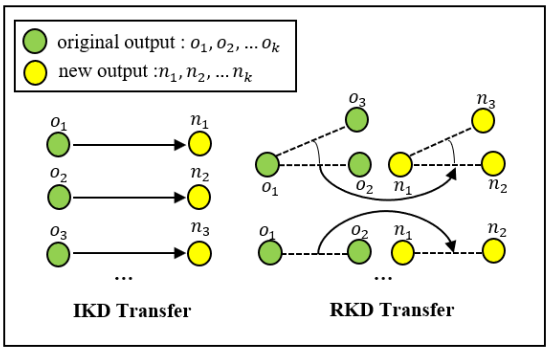
\includegraphics[width=\linewidth]{6rkd.png}

        {\tiny Figure-4: IKD transfers the knowledge point to point (original to new) while RKD transfers the structural relations (adjacency) of output}
    \end{columns}

    \vspace{0.3em}
    \begin{block}{}
        Building the Relation Graph require training at each incremental sessions 
    \end{block}

\end{frame}



\begin{frame}{Literature Review: Semantic Knowledge Distillation [4](CVPR, 2021)}

    \begin{columns}[c]
        \column{0.4\textwidth}
        \vspace{0.4em}
        {\footnotesize
        \begin{itemize}
            \item Predicts a fixed-length \textbf{semantic word vector} for each image. A novel class only needs \emph{its} word vector
            \item Base classes' word vectors are grouped together using k-means
            \item The idea is reusing knowledge from these semantically-related base-class word vectors
            \item An attention module learns how much to use each specialist embedding and combines them into the final representation
            \item Use these semantic knowledge via distillation to learn new classes
        \end{itemize}
        }


        \column{0.6\textwidth}
        \centering
        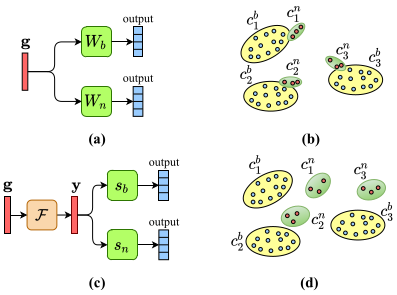
\includegraphics[height=4.1cm]{7wordvec.png}

        {\tiny Figure-5: Semantically-guided network with vectors for well-separated base-novel classes}

        \vspace{0.1em}
        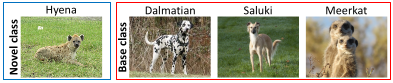
\includegraphics[width=0.9\linewidth]{9skd.png}

        {\tiny Figure-6: Novel class Hyena in presence of shared semantics (face, 4-ft height, body-shape, short-tail), helps classifying it and not to forget similar base classes (Dalmatian, Saluki, Meerkat)}
    \end{columns}

\end{frame}


\begin{frame}{Literature Review: FACT (ForwArd Compatible Training) [5](CVPR, 2022)}

    \begin{columns}[c]
        \column{0.4\textwidth}
        {\footnotesize
        \begin{itemize}
            \item In tradiotional knowledge-distillation, learn better base representation, then model learns to behave similarly at each incremental session (backward compatible)
            \item Instead of creating 5 prototypes from 5 base classes, create virtual class prototypes reserving spaces for future novel class (\textbf{forward compatible})
            \item Intuition is that interpolations between clusters (mixture of classes: e.g., dog-cat mix) leads to low-confidence (possible future-class) regions (\textbf{prototype forcasting})
        \end{itemize}
        }

        \column{0.6\textwidth}
        \centering
        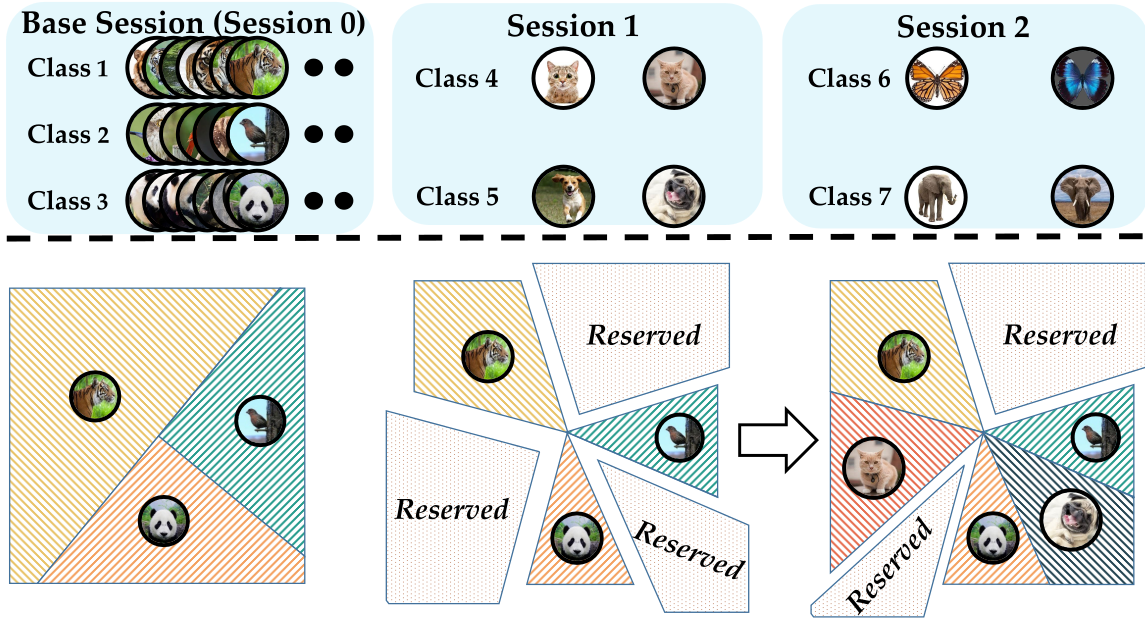
\includegraphics[width=\linewidth]{fwdc.png}

        {\tiny Figure-7: Traditional training vs reserved embedding space for novel classes in Forward Compatible training}
    \end{columns}

    \vspace{0.3em}
    \begin{block}{}
        Reserving spaces in feature space while creating virtual prototypes require substantial base classifier training using forward compatible loss
    \end{block}

\end{frame}


\begin{frame}{Literature Review: Semantic-Aware Virtual Contrastive Constraint [6](CVPR, 2023)}

    \begin{columns}[c]
        \column{0.44\textwidth}
        \vspace{0.4em}
        {\footnotesize
        \begin{itemize}
                \item "Better separation between base classes" leads to better ability to incorporate novel classes
                \item Classification and Contrastive loss are optimized in fantasy space (I don't have the future classes. But I can create additional semantic variations of the classes I do have)
                \item 12 augmentation (2 or 4-fold rotation x 3 color permutations) transformation on base classes; virtual class and fantasy label space for structuring huge empty spots in feature space
        \end{itemize}
        }

        \column{0.59\textwidth}
        \centering
        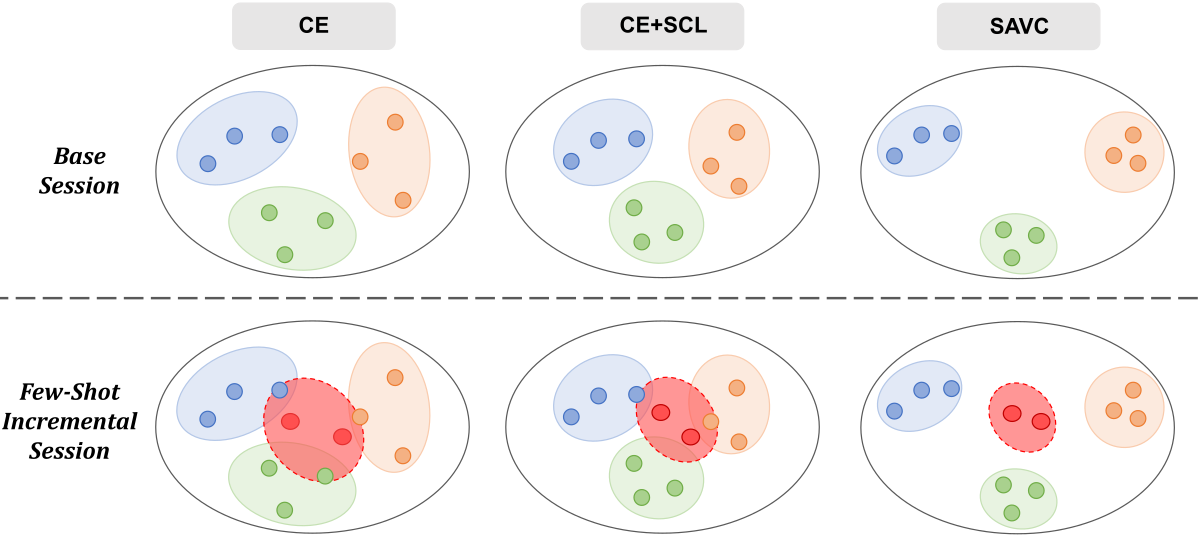
\includegraphics[width=0.82\linewidth]{savc1.png}

        \vspace{0.15em}
        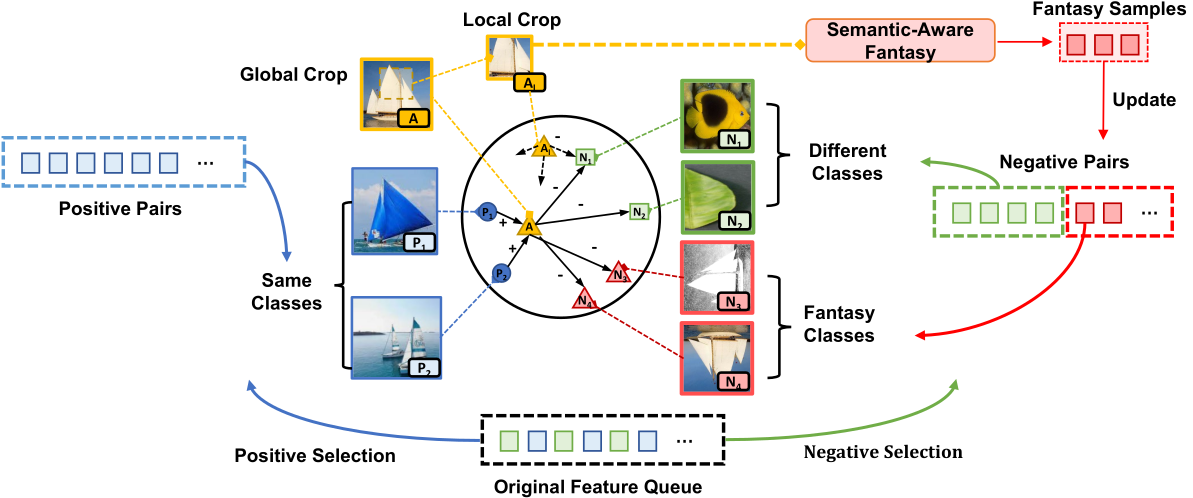
\includegraphics[width=0.82\linewidth]{savc2.png}

        {\tiny Figure-8: Embedding spaces comparison on different methods and semantic-aware virtual fantasy space}
    \end{columns}

\end{frame}

\begin{frame}{Towards Training Free FSCIL [7](CVPR, 2025)}

    \begin{columns}[c]
        \column{0.47\textwidth}
        {\footnotesize
        \begin{itemize}
            \item Prior methods solves plasticity-stability tradeoff via either both base and incremental session training or only base training and frozen support set
            \item Continual fine-tuning paradigm utilizes limited samples to continuously update the model, enhancing its plasticity.(\textbf{SKD, CEC, RKD,})
            \item Incremental-session freezing focuses on learning representations during base task, generalized to incremental tasks (\textbf{SAVC, FACT, TEEN})
        \end{itemize}
        }

        \column{0.52\textwidth}
        \centering
        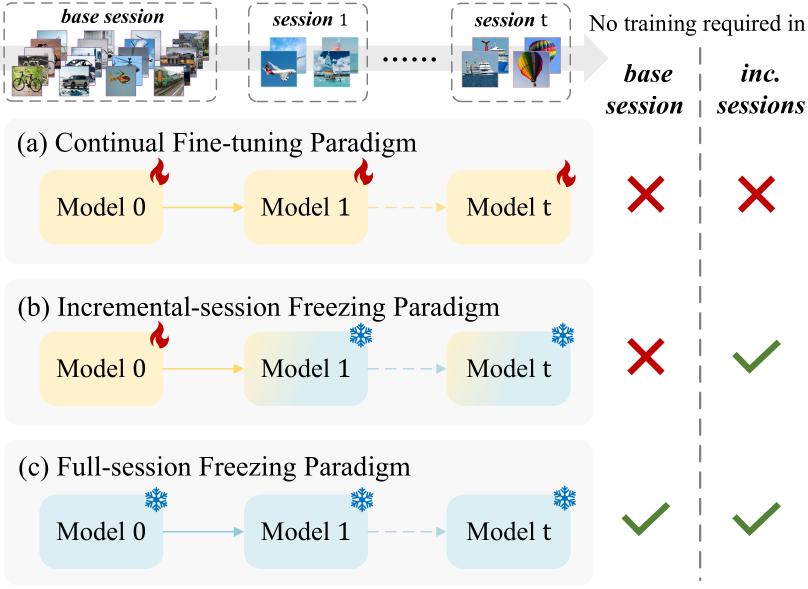
\includegraphics[width=\linewidth]{bimc.png}
    \end{columns}

    \vspace{0.3em}
    \begin{block}{}
        Both require additional training to adapt to new tasks (resource efficiency? model adaptability?)
    \end{block}

\end{frame}

\begin{frame}{Literature Review: Bi-Level Modality Calibration (BiMC) [7](CVPR, 2025)}

    \centering
    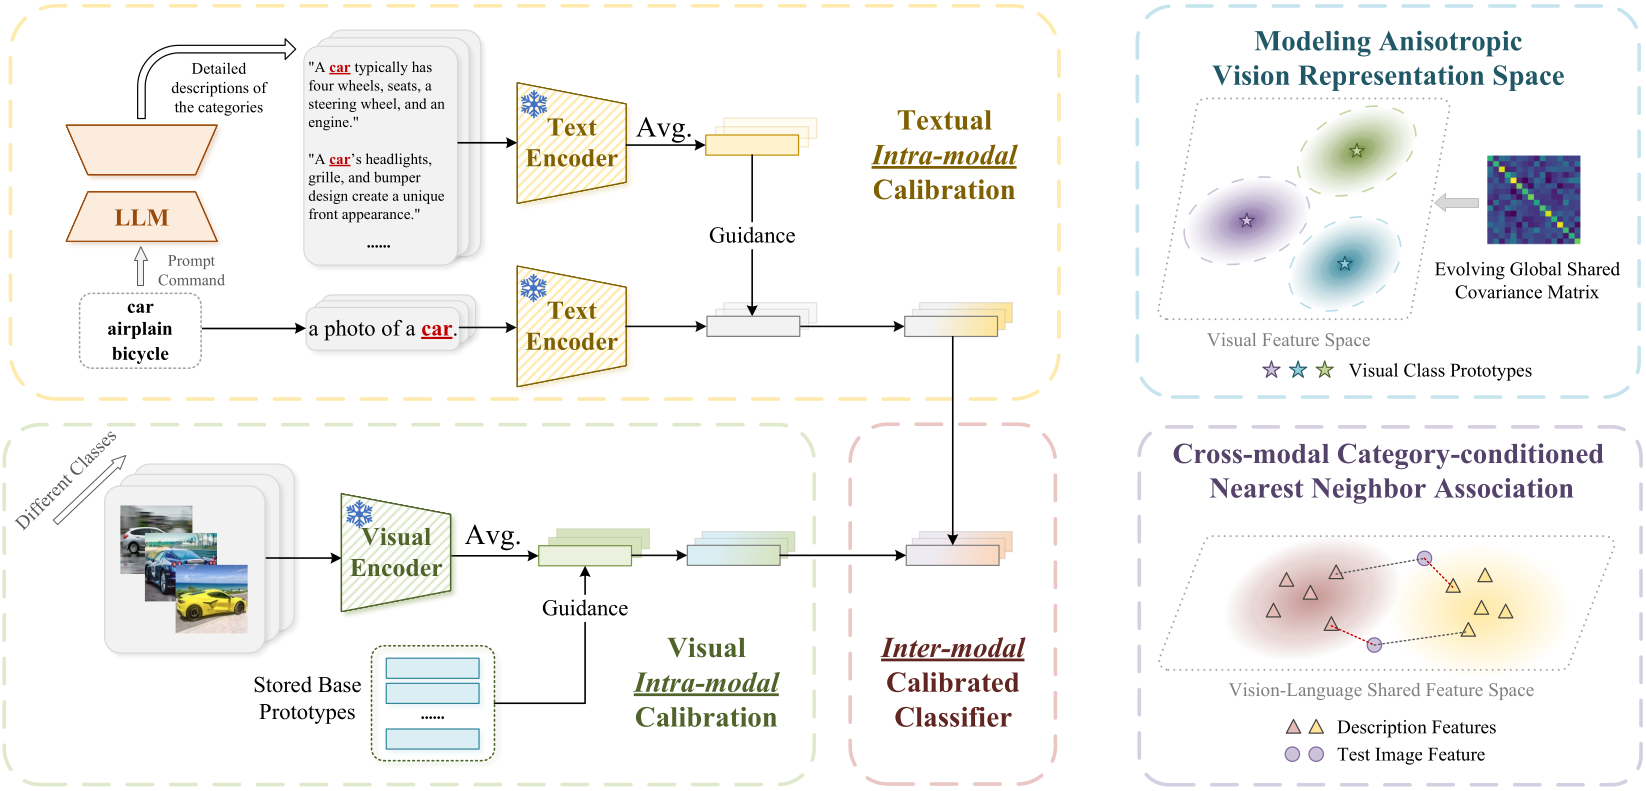
\includegraphics[width=0.92\linewidth]{bical.png}

    {\tiny Figure-9: Bi-Level Modality Calibration Framework with globally shared covariance metric for visual feature modeling and category-conditioned nearest-neighbor scoring}

\end{frame}


\begin{frame}{Training-Free FSCIL: Everything so far...}
        \centering
        \begin{block}{Limitations of calibration in BiMC}
        \begin{itemize}
            \item \textbf{Geometric} Only utilizing visual signals from CLIP is not suffiecient 
            \item \textbf{Statistical} Novel prototypes are estimated only from few support images. No utilization of unlabeled query batches.
        \end{itemize}
        \end{block}

        \vspace{2.5em}

        \centering
        \begin{block}{Our research questions}
            \begin{itemize}
                \item Can we \textbf{increase the visual feature space} for more refined prototype and leave room for novel class prototypes without training?
                \item Can we rectify noisy novel-alike prototype after base session?
                \item Can we further increase the inter-class distance and reduce intra-class gap (more reserved space)? 
            \end{itemize}
        \end{block}
\end{frame}


% \begin{frame}{Motivation}

%     \vspace{1.5em}
%     \begin{enumer        \begin{itemize}
%         \item \textbf{Geometric} Adding a self-supervised visual encoder (DINOv2), to introduce another visual space that is qualitatively different from CLIP's
%         \item \textbf{Statistical} Updating only DINOv2 novel prototypes through a precision-favoring gate driven by the calibrated posterior.
%         \item \textbf{Novel prototype refinement} Discriminative prompt based rerouting the novel prototypes as novel confusability guard.
%     \end{enumerate}
% \end{frame}

\begin{frame}{Overview of Proposed Methodology}

    \begin{block}{}
        Frozen FSCIL is fundamentally a \textbf{three-level calibration problem}, added with prototype refinement strategies using qury batches and textual evidence.
    \end{block}

    \vspace{2em}

    \begin{itemize}
            \item[$\Rightarrow$] \textbf{Inter-model calibration} with CLIP's share feature to produce stronger, complementary visual feature space (DINOv2) and \textbf{prototype-score calibration}

        \vspace{1em}
        
            \item[$\Rightarrow$] \textbf{Novel-mass gate} for novel prototype refinement utilizing \textbf{unlabeled query batch images}

        \vspace{1em}
        
            \item[$\Rightarrow$] \textbf{Pairwise discriminative prompt matrix} to add a very little bias on calculated prototype 
    \end{itemize}
\end{frame}


\begin{frame}{Methodology: Tri-Level Modality Calibration}

    \begin{columns}[c]
        \column{0.32\textwidth}
            {\footnotesize
            \begin{enumerate}
                \item Extract per class normalized visual features from both frozen encoder
                \item Build semantic prototype using CLIP's text encoder
                \item Inter-model visual calibration between CLIP and DINOv2: calculates each encoder's class-wise similarity scores, then combine scores
                \item Finally, combine both semantic and visual evidence scores
            \end{enumerate}
            }
            
            \vspace{2em}
            \footnote{\hyperlink{appendix}{see Appendix for detailed formulation}}

        \column{0.63\textwidth}
        \centering
        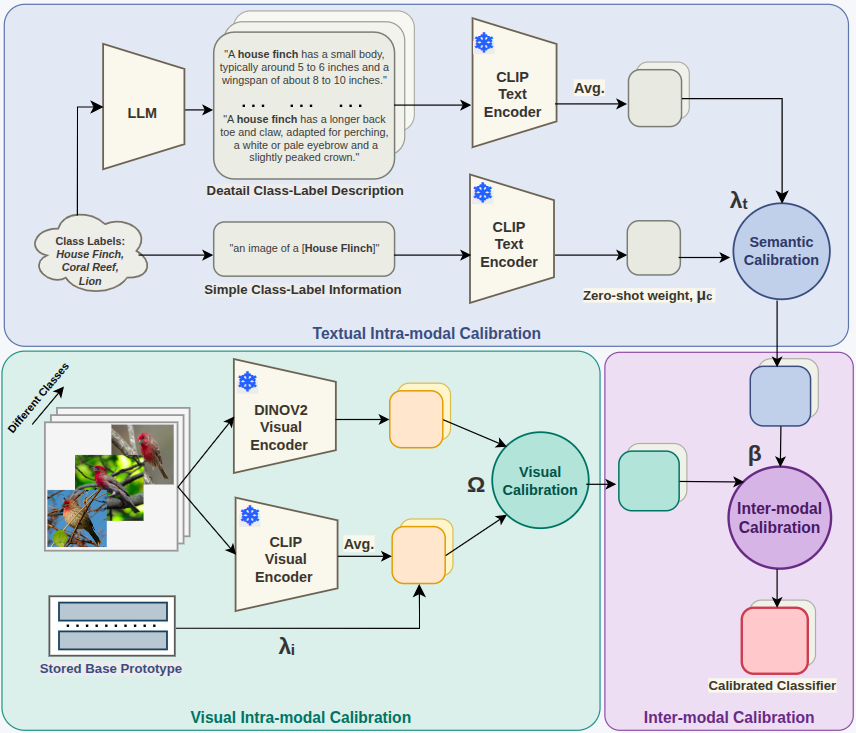
\includegraphics[width=0.92\linewidth]{tric.png}
    \end{columns}

\end{frame}


\begin{frame}{Methodology: Query Prototype Refinement}

    \begin{columns}[c]
        \column{0.35\textwidth}
        {\footnotesize
            \begin{enumerate}
                \item Select reliable (noise-free) unlabeled query images and group them by predicted novel class
                \item Compute a probability-weighted query prototype (more influence to higher-confidence queries)
                \item Keep unreliable classes unchanged and blend reliable ones with noisy novel 5-shot prototypes
            \end{enumerate}
        }

            \vspace{4em}
            \footnote{\hyperlink{appendix}{see Appendix for detailed formulation}}

        \column{0.65\textwidth}
        \centering
        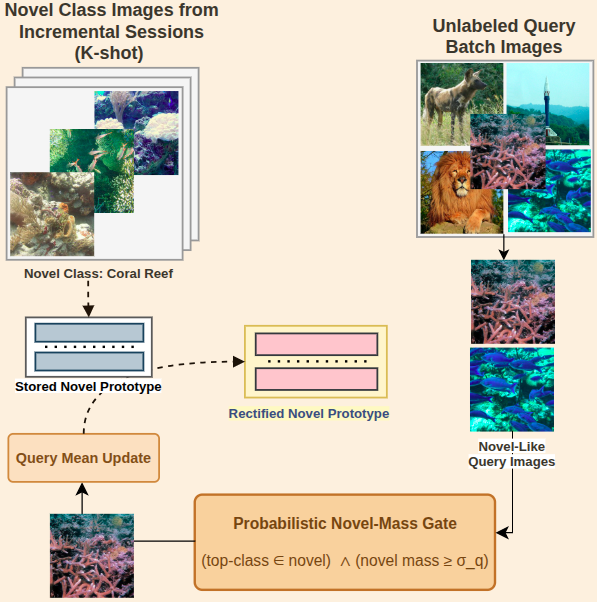
\includegraphics[height=7.6cm]{qpr.png}

    \end{columns}

\end{frame}

\begin{frame}{Methodology: Class Pairwise Discriminative Prompt matrix}

    \begin{block}{}
        \footnotesize
        For every class pair $(i,j)$, matrix stores $k{=}3$ prompts describing class $i$ \emph{against} class $j$; each prompt targets a \textbf{different} discriminative attribute, the average text embedding $N_{i,j}$ spans the discriminative subspace rather than repeating one cue.
    \end{block}

    \vspace{0.2em}
    \begin{columns}[c]
        \column{0.63\textwidth}
        {\scriptsize
        \begin{exampleblock}{\emph{mini}ImageNet \quad $M_{\text{Saluki},\,\text{Ibizan hound}}$}
            \begin{itemize}\setlength{\itemsep}{0pt}
                \item[1.] ``a photo of a Saluki, whose long \textbf{feathered ears hang down} unlike the erect ears of an Ibizan hound''
                \item[2.] ``a photo of a Saluki, with \textbf{silky fringed fur} instead of the short hard coat of an Ibizan hound''
                \item[3.] ``a photo of a Saluki, showing a \textbf{dark nose and dark eyes} unlike a pink nosed Ibizan hound''
            \end{itemize}
        \end{exampleblock}

        \vspace{-0.3em}
        \begin{exampleblock}{CUB-200 \quad $M_{\text{Ring-billed Gull},\,\text{Herring Gull}}$}
            \begin{itemize}\setlength{\itemsep}{0pt}
                \item[1.] ``a photo of a Ring-billed Gull, notably \textbf{smaller and more delicate} than a Herring Gull''
                \item[2.] ``a photo of a Ring-billed Gull, with \textbf{yellow legs} rather than the pink legs of a Herring Gull''
                \item[3.] ``a photo of a Ring-billed Gull, its bill circled by a \textbf{black ring without any red spot}''
            \end{itemize}
        \end{exampleblock}
        }

        \column{0.34\textwidth}
        \centering
        \begin{minipage}[t]{0.47\linewidth}\centering
            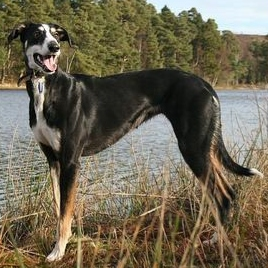
\includegraphics[height=1.5cm]{saluki.jpg}\\[0.1em]
            {\tiny Dog-class: Saluki}
        \end{minipage}\hfill
        \begin{minipage}[t]{0.47\linewidth}\centering
            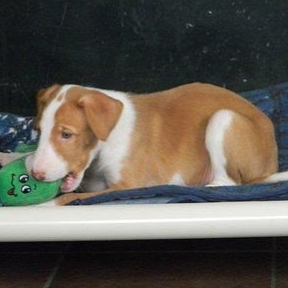
\includegraphics[height=1.5cm]{Ibizan_hound.jpg}\\[0.1em]
            {\tiny Dog-class: Ibizan Hound}
        \end{minipage}

        \vspace{0.3em}
        \begin{minipage}[t]{0.47\linewidth}\centering
            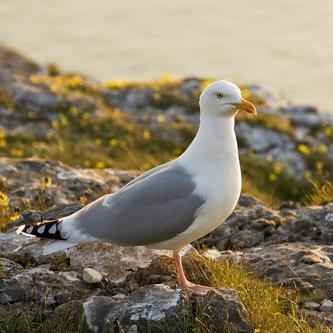
\includegraphics[height=1.5cm]{hering_gull.jpg}\\[0.1em]
            {\tiny Bird-class: Herring Gull}
        \end{minipage}\hfill
        \begin{minipage}[t]{0.47\linewidth}\centering
            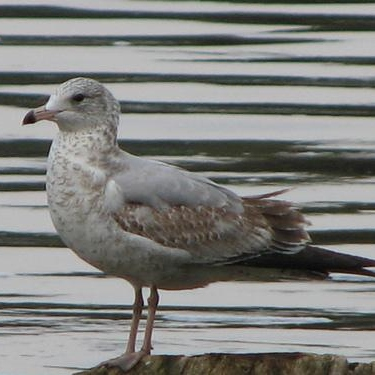
\includegraphics[height=1.5cm]{ring_billed_gull.jpg}\\[0.1em]
            {\tiny Bird-class: Ring-billed Gull}
        \end{minipage}
        
        \vspace{1em}
        
        {\tiny Figure-10: Sample images from miniImageNet and CUB200}

    \end{columns}

\end{frame}

\begin{frame}{Methodology: Discriminative Prompt Rerouting (DPR)}

    \begin{columns}[c]
        \column{0.28\textwidth}
        {\scriptsize
        \hrule height 0.9pt
        \vspace{3pt}
        \textbf{Algorithm} 
        \vspace{3pt}
        \hrule height 0.4pt
        \vspace{4pt}
        \begin{enumerate}
            \setlength{\itemsep}{5pt}
            \item Compute pairwise prototype similarity $S_{i,j}$ and new prototype vector of class i, $N_{i,j}$ following discriminative embeddings
            \item Pick the most confusable unvisited pair $(a,b)$ with $S_{a,b} > r_{th}$
            \item Compute similarity of the \emph{new} prototype to every other class $i$
            \item Guard 1: keep only if $S_{a,b} > tmp_{a',b'}$
            \item Guard 2: keep only if similarity to all other classes drops by $< 0.1$
            \item Reroute prototype by updating $T'_a$, $T'_b$ independently; until no pair exceeds $r_{th}$
        \end{enumerate}
        \vspace{4pt}
        \hrule height 0.9pt
        }


        \column{0.73\textwidth}
        \centering
        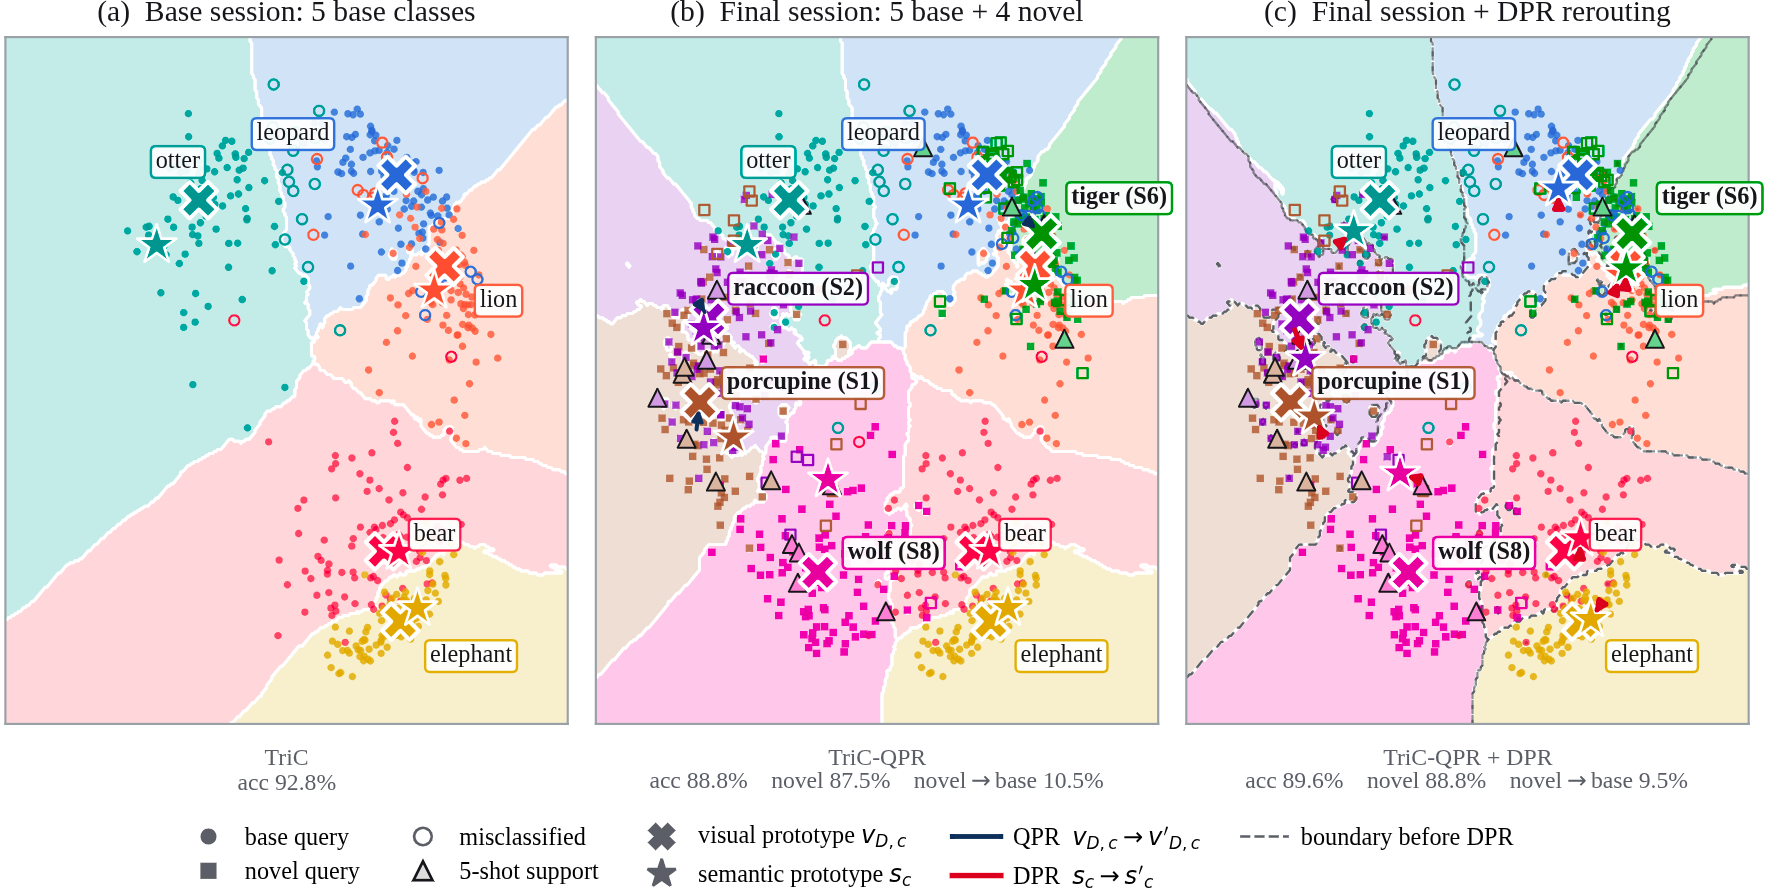
\includegraphics[width=\linewidth]{dprreroute.png}

        \vspace{1em}

        {\tiny Figure-11: t-SNE heatmap of Prototype update with class-wise Discriminative Prompt}

    \end{columns}

\end{frame}


\begin{frame}{Results}

    {\tiny {[All values experimented with train-val-test split in \textbf{20 seeds} avg*]}}

    \vspace{0.3em}
    \centering
    \resizebox{0.8\linewidth}{!}{%
    \begin{tabular}{lc ccccccccc cc}
    \toprule
     & & \multicolumn{9}{c}{Accuracy in each session (\%) $\uparrow$} & & \\
    \cmidrule(lr){3-11}
    Method & Modality & $A_0$ & $A_1$ & $A_2$ & $A_3$ & $A_4$ & $A_5$ & $A_6$ & $A_7$ & $A_8$ & Avg. $\uparrow$ & PD $\downarrow$ \\
    \midrule
    CLIP zero-shot & L & 74.77 & 73.12 & 72.56 & 71.08 & 70.46 & 70.41 & 70.58 & 70.06 & 68.93 & 71.33 & 5.84 \\
    Visual prototype (CLIP) & V & 75.88 & 72.78 & 71.01 & 68.52 & 66.55 & 64.84 & 64.12 & 62.71 & 61.03 & 67.49 & 14.85 \\
    TEEN & V & 75.88 & 73.00 & 71.39 & 68.88 & 67.14 & 65.41 & 64.94 & 63.44 & 61.84 & 67.99 & 14.04 \\
    FeCAM & V & 81.38 & 78.28 & 76.93 & 74.55 & 72.91 & 71.81 & 71.26 & 69.80 & 68.32 & 73.92 & 13.06 \\
    BiMC & V-L & 79.70 & 77.97 & 77.29 & 75.35 & 74.76 & 74.39 & 74.34 & 73.55 & 72.50 & 75.54 & 7.20 \\
    BiMC Ens. & V-L & 81.98 & 79.74 & 78.84 & 77.00 & 76.11 & 75.68 & 75.33 & 74.61 & 73.18 & 76.94 & 8.80 \\
    CLIP visual only & V & 75.90 & 72.74 & 70.97 & 68.31 & 66.54 & 65.49 & 64.94 & 63.73 & 62.20 & 67.87 & 13.70 \\
    DINO visual only & V & 89.63 & 87.87 & 87.21 & 85.16 & 85.22 & 84.90 & 84.92 & 84.57 & 83.34 & 85.87 & 6.29 \\
    \textsc{Ours} & V-L & 90.90 & 89.78 & 89.42 & 88.04 & 88.17 & 87.98 & 88.12 & 87.91 & 87.13 & \textbf{88.61} & \textbf{3.77} \\
    \bottomrule
    \end{tabular}}

    \vspace{0.5em}

    \centering
    \resizebox{0.8\linewidth}{!}{%
    \begin{tabular}{lc ccccccccccc cc}
    \toprule
     & & \multicolumn{11}{c}{Accuracy in each session (\%) $\uparrow$} & & \\
    \cmidrule(lr){3-13}
    Method & Modality & $A_0$ & $A_1$ & $A_2$ & $A_3$ & $A_4$ & $A_5$ & $A_6$ & $A_7$ & $A_8$ & $A_9$ & $A_{10}$ & Avg. $\uparrow$ & PD $\downarrow$ \\
    \midrule
    CLIP zero-shot & L & 66.38 & 64.05 & 62.71 & 59.07 & 59.24 & 59.27 & 57.76 & 56.69 & 55.46 & 55.19 & 55.73 & 59.23 & 10.65 \\
    Visual prototype (CLIP) & V & 81.42 & 78.78 & 77.43 & 74.22 & 72.91 & 71.59 & 70.65 & 69.97 & 68.79 & 68.93 & 68.80 & 73.04 & 12.62 \\
    TEEN & V & 81.42 & 79.16 & 77.49 & 74.60 & 73.26 & 71.75 & 70.68 & 70.21 & 68.90 & 69.28 & 69.12 & 73.26 & 12.30 \\
    FeCAM & V & 82.26 & 79.48 & 77.76 & 74.68 & 72.86 & 71.10 & 69.92 & 69.17 & 67.61 & 67.89 & 67.40 & 72.74 & 14.86 \\
    BiMC & V-L & 82.16 & 79.99 & 79.04 & 76.10 & 75.07 & 74.04 & 73.13 & 73.08 & 71.88 & 72.26 & 72.25 & 75.36 & 9.91 \\
    BiMC Ens. & V-L & 83.00 & 81.01 & 79.83 & 76.96 & 75.84 & 74.73 & 73.86 & 73.47 & 72.26 & 72.61 & 72.68 & 76.02 & 10.32 \\
    CLIP visual only & V & 81.63 & 79.14 & 77.49 & 74.24 & 73.26 & 71.68 & 70.81 & 70.03 & 68.53 & 68.72 & 68.47 & 73.09 & 13.16 \\
    DINO visual only & V & 86.35 & 85.19 & 84.66 & 83.67 & 83.68 & 82.34 & 82.72 & 83.28 & 83.14 & 83.65 & 84.01 & 83.88 & 2.34 \\
    \textsc{Ours} & V-L & 87.64 & 86.58 & 86.23 & 85.40 & 85.66 & 84.46 & 84.84 & 85.32 & 85.16 & 85.62 & 85.97 & \textbf{85.72} & \textbf{1.67} \\
    \bottomrule
    \end{tabular}}

    \vspace{0.3em}
    {\footnotesize \centering Table-1: Session-wise comparison on CIFAR100 and CUB200\par}

\end{frame}



\begin{frame}{Result Analysis: Tri level Calibration Impact}

    \centering
    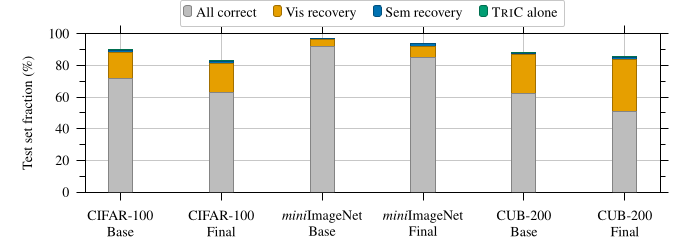
\includegraphics[width=0.67\linewidth]{tricImpact.png}

    {\tiny Figure-12: Per-query behavior of TRIC’s inter-modal calibration at base and final sessions}
    
    % \normalsize

    \vspace{0.15em}
    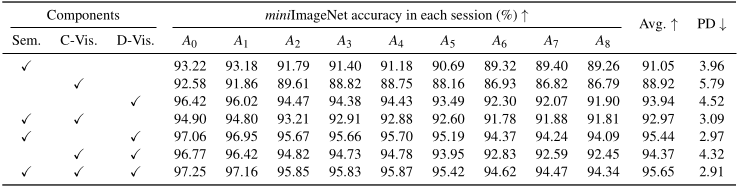
\includegraphics[width=0.75\linewidth]{tricImpactComp.png}

    {\tiny Table-2: Component ablation of Calibration on miniImageNet with Semantic, CLIP-visual, and DINOv2-visual branches}

\end{frame}

\begin{frame}{Result Analysis: QPR Impact}

    \centering
    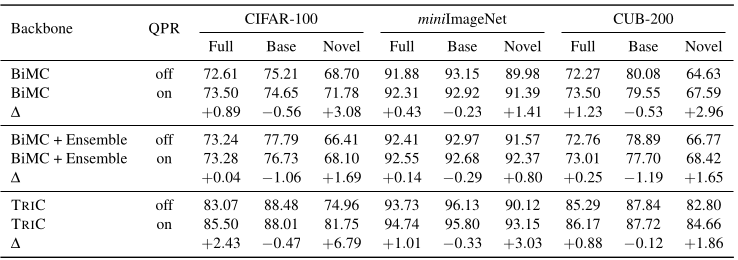
\includegraphics[width=0.56\linewidth]{qprImpact.png}

    {\tiny Table-3: QPR Accuracy Analysis, Full/Base/Novel accuracy across different backbones}
    \normalsize

    \vspace{0.2em}
    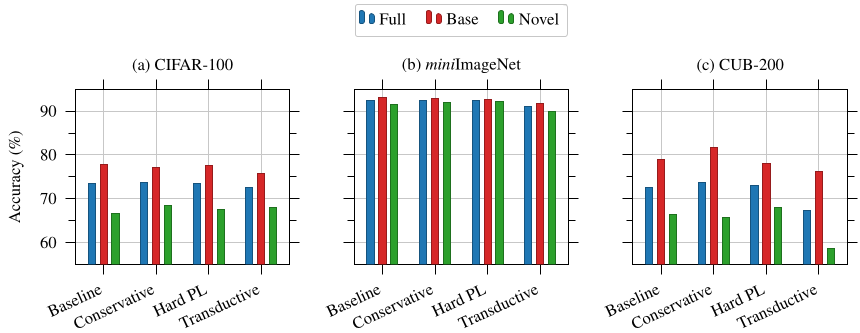
\includegraphics[width=0.6\linewidth]{qprBimc.png}

    {\tiny Figure-13: QPR ablation on different gating mechanisms (Baseline, Conservative, Hard PL, Transductive) over BiMC}

\end{frame}

\begin{frame}{Result Analysis: DPR Impact}

    \centering
    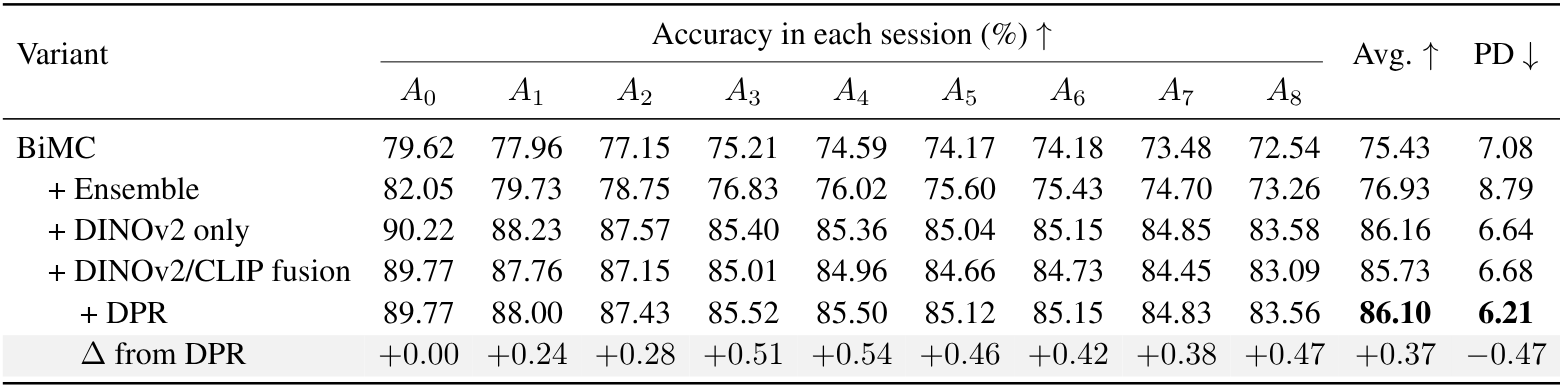
\includegraphics[width=0.57\linewidth]{dprImpact.png}

    {\tiny Table-4: DPR ablation on per-session accuracy on each module with refined prototype in CIFAR100}
    \normalsize

    \vspace{0.3em}
    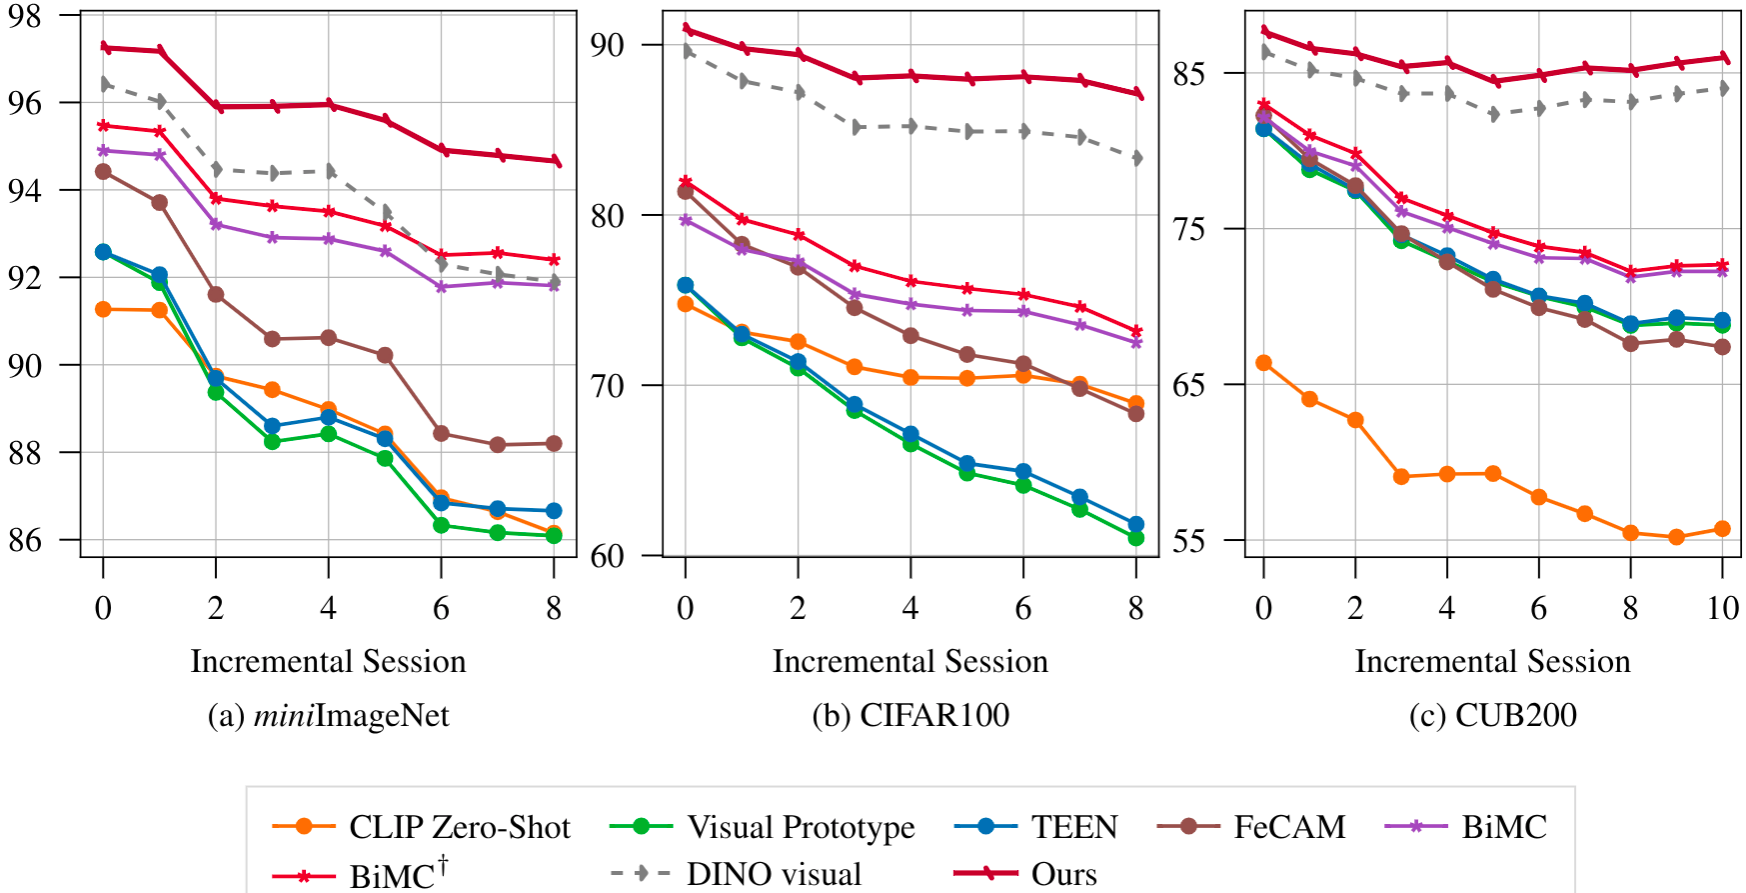
\includegraphics[width=0.56\linewidth]{finalres.png}

    {\tiny Figure-14: Final session-wise accuracy across all datasets: Ours vs Other methods [8](NeurIPS, 2023) [9](NeurIPS, 2024)}

\end{frame}

% \begin{frame}{Ablation on Updated Prototype and Conclusion}
   

% \end{frame}


\begin{frame}{Conclusion}

        We propose a training-free approach to few-shot class-incremental learning where,
        \vspace{0.7em}
        \begin{itemize}
            \setlength{\itemsep}{1pt}
            \item Tri level calibration with stronger DinoV2 visual space is challenging as averaging incompatible embedding spaces is geometrically meaningless, so we calibrated [CLS] scores with normalized cosine distance
            \vspace{1em}
            \item QPR incorporates unlabeled query batch to rectify noisy novel prototypes, without leaking base-class noise which is well-motivated by the need for precision over coverage
            \vspace{1em}
            \item DPR reroutes only the most confusing class pair prototypes after calibration, thus creating virtual prototypes with class-specific discriminative-prompt. Update only when no other class's similarity gets worse because of rerouting
        \end{itemize}

\end{frame}

\begin{frame}{Limitations}
    \begin{columns}[t]
        \column{0.42\textwidth}
        \centering
        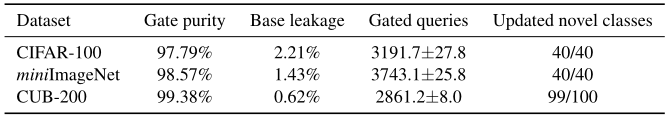
\includegraphics[width=\linewidth]{protoupdate.png}

        \footnotesize (A) Prototype update statistics per query
        \normalsize

        \column{0.52\textwidth}
        \centering
        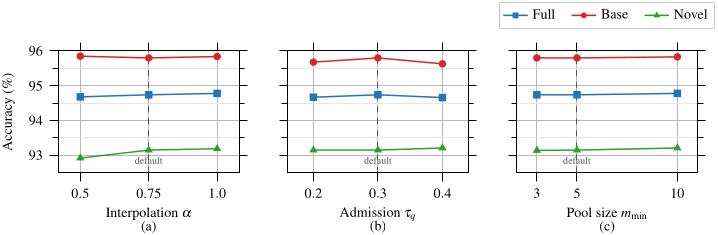
\includegraphics[width=\linewidth]{hyperparam.png}

        \footnotesize (B) Hyperparameter sensitivity test on \emph{mini}ImageNet, varied one at a time with default $(\alpha, \tau_q, m_{\min}) = (0.75, 0.3, 5)$
        \normalsize
    \end{columns}

    \vspace{0.1em}
{\footnotesize
\begin{alertblock}{}
        Limitations of our methods:
        \begin{itemize}
            \setlength{\itemsep}{1pt}
            \item QPR is transductive and may depend on query-batch composition. 
            \item DPR depends on the quality of LLM generated discriminative prompts. 
            \item Multiple coefficients are introduced, too much knob (not generalized). The hyperparameter selection is empirical. 
        \end{itemize}
    Although, In our defence:
    \begin{itemize}
            \setlength{\itemsep}{1pt}
            \item QPR and DPR both module may not guarantee prototype update in all cases but on avg it performs better than baseline (20 seeds results show at least as good as baseline, on avg even better!)
            \item Hyperparameter sensitivity test shows that the effect of its change is negligible 
    \end{itemize}
    
        \end{alertblock}
}
\end{frame}


\begin{frame}{References}
    \textbf{Works Cited in This Presentation}

    \vspace{0.4em}
    {\scriptsize
    \begin{enumerate}
        \setlength{\itemsep}{3pt}
        \item X. Tao, X. Hong, X. Chang, S. Dong, X. Wei, and Y. Gong, ``Few-shot class-incremental learning,'' in \textit{Proc. IEEE/CVF Conf. on Computer Vision and Pattern Recognition (CVPR)}, 2020.
        \item C. Zhang, N. Song, G. Lin, Y. Zheng, P. Pan, and Y. Xu, ``Few-shot incremental learning with continually evolved classifiers,'' in \textit{CVPR}, 2021.
        \item S. Dong, X. Hong, X. Tao, X. Chang, X. Wei, and Y. Gong, ``Few-shot class-incremental learning via relation knowledge distillation,'' in \textit{AAAI}, 2021.
        \item A. Cheraghian, S. Rahman, P. Fang, S. K. Roy, L. Petersson, and M. Harandi, ``Semantic-aware knowledge distillation for few-shot class-incremental learning,'' in \textit{CVPR}, 2021.
        \item Z. Song, Y. Zhao, Y. Shi, P. Peng, L. Yuan, and Y. Tian, ``Learning with fantasy: semantic-aware virtual contrastive constraint for few-shot class-incremental learning,'' in \textit{CVPR}, 2023.
        \item D.-W. Zhou, F.-Y. Wang, H.-J. Ye, L. Ma, S. Pu, and D.-C. Zhan, ``Forward compatible few-shot class-incremental learning,'' in \textit{CVPR}, 2022.
        \item Y. Chen, T. Ding, L. Wang, J. Huo, Y. Gao, and W. Li, ``Enhancing few-shot class-incremental learning via training-free bi-level modality calibration,'' in \textit{CVPR}, 2025.
        \item Q.-W. Wang, D.-W. Zhou, Y.-K. Zhang, D.-C. Zhan, and H.-J. Ye, ``Few-shot class-incremental learning via training-free prototype calibration,'' in \textit{NeurIPS}, 2023.
        \item D. Goswami, Y. Liu, B. Twardowski, and J. van de Weijer, ``FeCAM: exploiting the heterogeneity of class distributions in exemplar-free continual learning,'' in \textit{NeurIPS}, 2024.
    \end{enumerate}
    }
\end{frame}



\begin{frame}{Appendix: Equations and Formulas in Methodology}
        \hypertarget{appendix}{}
        \begin{columns}[t]
        \column{0.49\textwidth}
        \begin{alertblock}{TriC}
        \tiny
        \begin{align*}
            \mathcal{C}_{\le t} &= \bigcup_{s=0}^{t}\mathcal{C}^{(s)}, \;\; \mathcal{C}_b=\mathcal{C}^{(0)}, \;\; \mathcal{C}_n=\mathcal{C}_{\le t}\setminus\mathcal{C}_b \\[6pt]
            \text{norm}(\mathbf{u}) &= \tfrac{\mathbf{u}}{\|\mathbf{u}\|_2}, \;\; q_C(\mathbf{x})=\text{norm}(f_I(\mathbf{x})), \;\; q_D(\mathbf{x})=\text{norm}(f_D(\mathbf{x})) \\[6pt]
            w_c &= \text{norm}(f_T(\pi_c)), \;\; \bar{z}_c = \text{norm}\Big(\tfrac{1}{n_c}\textstyle\sum_{r=1}^{n_c} z_{c,r}\Big) \\[6pt]
            v_{C,c} &= \text{norm}\Big(\tfrac{1}{m_c}\textstyle\sum_{j} q_C(\mathbf{x}_{c,j})\Big), \;\; v_{D,c} = \text{norm}\Big(\tfrac{1}{m_c}\textstyle\sum_{j} q_D(\mathbf{x}_{c,j})\Big) \\[6pt]
            s_c &= \text{norm}\big((1-\lambda_T)w_c + \lambda_T \bar{z}_c\big) \\[6pt]
            \ell_c^S(\mathbf{x}) &= q_C(\mathbf{x})^\top s_c \\[6pt]
            \ell_c^V(\mathbf{x}) &= \omega\, q_D(\mathbf{x})^\top v_{D,c} + (1-\omega)\, q_C(\mathbf{x})^\top v_{C,c} \\[6pt]
            \ell_c^F(\mathbf{x}) &= \beta \ell_c^S(\mathbf{x}) + (1-\beta)\ell_c^V(\mathbf{x}), \;\; p_{\text{TriC}}(c\mid \mathbf{x}) = \dfrac{\exp(\rho\, \ell_c^F(\mathbf{x}))}{\sum_{k\in\mathcal{C}_{\le t}} \exp(\rho\, \ell_k^F(\mathbf{x}))}
        \end{align*}
        \end{alertblock}

        \column{0.45\textwidth}
        \begin{alertblock}{QPR}
        \tiny
        \begin{align*}
            \hat{y}(\mathbf{x}) &= \arg\max_{k\in\mathcal{C}_{\le t}} p^*(k\mid\mathbf{x}), \;\; m_n(\mathbf{x}) = \sum_{k\in\mathcal{C}_n} p^*(k\mid\mathbf{x}) \\[0pt]
            \mathcal{G}_c &= \{\mathbf{x}\in\mathcal{U}_t : \hat{y}(\mathbf{x})=c,\; m_n(\mathbf{x})\ge \tau_q\}, \;\; c\in\mathcal{C}_n \\[0pt]
            a_c(\mathbf{x}) &= \dfrac{p^*(c\mid\mathbf{x})}{\sum_{\mathbf{x}'\in\mathcal{G}_c} p^*(c\mid\mathbf{x}')}, \;\; \tilde{v}_{D,c} = \text{norm}\Big(\textstyle\sum_{\mathbf{x}\in\mathcal{G}_c} a_c(\mathbf{x})\, q_D(\mathbf{x})\Big) \\[0pt]
            v'_{D,c} &= \begin{cases}
                \text{norm}\big((1-\alpha)v_{D,c}+\alpha\tilde{v}_{D,c}\big), & c\in\mathcal{C}_n,\ |\mathcal{G}_c|\ge m_{\min} \\[0pt]
                v_{D,c}, & \text{otherwise}
            \end{cases}
        \end{align*}
        \end{alertblock}

        \vspace{0.05em}
        \begin{alertblock}{DPR}
        \tiny
        \begin{align*}
            tmp_{a',i} &= \cos(T'_a, T_i) \\[0pt]
            T'_a &= T_a + \alpha D_{a\to b}, \;\; T'_b = T_b + \alpha D_{b\to a} \\[0pt]
            &\left(\forall_{\substack{i \ne a \\ i \ne b}} S_{a,i} - \forall_{\substack{i \ne a' \\ i \ne b'}} tmp_{a',i}\right) > -0.1
        \end{align*}
        \end{alertblock}
        \end{columns}

\end{frame}


\end{document}

